%!TEX root = start.TEX
\frame{\titlepage}

\AtBeginSection[]{
\begin{frame}
\frametitle{
	\begin{center}
	\vskip -0.8cm
	{\fontsize{13}{13.4}\selectfont{Modelo De Reconocimiento Automático De Señales De Tránsito Vehicular Mediante Aprendizaje Profundo De Redes Neuronales Convolucionales}}
	\end{center}
	\vskip -1cm
	}
	\tableofcontents[currentsection]
	\end{frame}
}

\frame{
\begin{abstract}
\justifying
%\begin{center}
 La presente investigación tiene por objetivo principal implementar un modelo basado en el aprendizaje profundo de redes neuronales convolucionales para reconocer automáticamente señales de tránsito vehicular usando técnicas de procesamiento de imágenes y fundamentos de inteligencia artificial.
  \vskip 0.2cm
  El proyecto se centra en un grupo de señales de Tránsito vehicular de Alemania y Perú, identificando 43 y 7 categorías respectivamente. Iniciando con  la adquisición de imágenes, se procedió realizar el procesamiento de estas con la finalidad de aumentar el conjunto de datos y poder ejecutar el aprendizaje profundo a través de diversos diseños de arquitecturas de redes neuronales convolucionales.
  \vskip 0.2cm
  Como resultado final, se obtuvo un modelo con buenos indicadores y resultados en el reconocimiento de señales de tránsito vehicular. De esta manera, se pretende contribuir en los esfuerzos de la industria automotriz en el campo de sistemas avanzados de asistencia al conductor así como también puede formar parte de diversos mecanismos que buscan dar soluciones a la inseguridad vial.
  \vskip 0.2cm
 	\begin{center} 
  {\bf Palabras claves:} aprendizaje profundo, redes neuronales convolucionales, procesamiento de imágenes.
	\end{center}
\end{abstract}
}

%-------------------------------------------------------------------------------------------------
%-------------------------------------------------------------------------------------------------
\section{Introducción}
	\frame{
	\begin{block}
	{\Large{Introducción}}
	\end{block}
	\vskip 0.5cm
	\begin{itemize}
		
		\item<1->Al conducir en carreteras congestionadas, a veces es difícil mantener los ojos en todas partes a la vez, comprobando el camino por delante, el tráfico venidero, lo que está detrás de usted, tratar de mantener la velocidad permitida; es por ello, que existen mecanismos destinados a reglamentar el tránsito, advertir o informar a los usuarios mediante palabras, sonidos o símbolos determinados.

		\item<2->La policía de tránsito o las {\bf señalizaciones vehiculares} que según sea el caso, en todos los países regulan el tránsito e informan al usuario sobre direcciones, rutas, destinos, así como dificultades existentes en las carreteras y previenen cualquier peligro que podría presentarse en la circulación vehicular.

	\end{itemize}
	}

	\frame{
	\begin{block}
	{\Large{Introducción}}
	\end{block}
	\vskip 0.5cm
	\begin{itemize}
		
		\item<1-> La inseguridad vial es un problema de interés mundial, según el último informe de la OMS (Organización Mundial de la salud) anualmente cerca de 1,3 millones de personas mueren alredor del mundo y entre 20 y 50 millones padecen traumatismos no mortales,\citep{OMS}. Son distintas las causas que conllevan a este problema, de las cuales las principales pueden ser la falta de concientización y educación vial.
	\end{itemize}
	}

	\frame{
	\begin{block}
	{\Large{Introducción}}
	\end{block}
	\vskip 0.5cm
	\begin{itemize}
		
		\item<1-> El Perú y la capital Lima se encuentran respectivamente en la lista de peores países y ciudades para conducir en America Latina, según el Índice Global de Satisfacción del Conductor \citep{CNN}, lo cual se ve reflejado en que los últimos años se ha incrementado el índice de mortandad originados por los accidentes de tránsito siendo las principales causas de los mismos el exceso de velocidad, estado de ebriedad del conductor y sobretodo el desacato a las señales de tránsito, todas ellas de responsabilidad directa del conductor del vehículo motorizado,\citep{SUTRAN}. 
		 
		\item<2-> Es por ello que trabajar en obtener vehículos más seguros es un factor fundamental para prevenir de alguna forma los accidentes de tránsito o reducir la probabilidad de que estos sean producidos, \citep{OMS}.
		
	\end{itemize}
	}

%-------------------------------------------------------------------------------------------------
%-------------------------------------------------------------------------------------------------

\section{Motivación}
	\frame{
	\begin{block}
	{\Large{Motivación}}
	\end{block}
	\vskip 0.2cm
	\begin{itemize}
		\item<1-> Para contribuir con lo antes mencionado, se han venido planteando formas que permitan la asistencia en el reconocimiento de señales de tránsito, la cual es un problema de clasificación multicategórica que comúnmente presenta desigualdades en las frecuencias de aparición de las categorías. Además, las señales de tránsito muestran una amplia gama de variaciones entre las clases en términos de color, forma, subconjuntos de clases que son muy similares entre sí y la presencia de símbolos, leyendas o texto. A esto es sumado, las grandes variaciones en las apariencias visuales debido a cambios de iluminación, oclusiones parciales, rotaciones, condiciones meteorológicas, escalamiento, etc. 

		\item<2-> Todo esto representa un reto para el reconocedor/clasificador de señales de tránsito vehicular y es por ello que se han venido realizando diversas investigaciones, donde esta forma parte de una de ellas.
	\end{itemize}
	}
%-------------------------------------------------------------------------------------------------
%-------------------------------------------------------------------------------------------------
\section{Formulación del problema}
	\frame{
	\begin{block}
	{\Large{Formulación del problema}}
	\end{block}
	\vskip 0.3cm
	 En este trabajo, se propone discutir el modelo de redes neuronales convolucionales basado en el problema del reconocimiento de imágenes para responder a la siguiente pregunta:
	 \vskip 0.3cm
	 \begin{center} 
	     \textbf{¿Cómo se puede reconocer de manera automática señales de tránsito vehicular?}
	 \end{center}
	}
%-------------------------------------------------------------------------------------------------
%-------------------------------------------------------------------------------------------------

\section{Importancia de la investigación} 
	\frame{
	\vskip -1cm
	\begin{block}
	{\Large{Importancia de la investigación - Justificación Académica}}
	\end{block}
	\vskip 0.3cm
	\begin{itemize}
	\item<1->  La importancia de esta investigación en el punto de vista de ciencias de la computación se justifica en poner en práctica los conocimientos adquiridos en la formación académica, siendo los más resaltables el tema de procesamiento de imágene e inteligencia artificial, con la finalidad de obtener un modelo robusto de redes neuronales convolucionales basadas en el aprendizaje profundo (deep learning) que permita el reconocimiento de señales de tránsito vehicular. 
	\vskip 0.15cm
	\item<2-> En este sentido, esta investigación se centra en un grupo de señales de Tránsito vehicular de Alemania y Perú, identificando 43 y 7 categorías respectivamente. Iniciando con la adquisición de imágenes, se procede a realizar el procesamiento de estas con la finalidad de aumentar el conjunto de datos y poder ejecutar el aprendizaje profundo a través de diferentes diseños de arquitecturas de redes neuronales convolucionales.
	\end{itemize}
	}

	\frame{
	\vskip -0.5cm
	\begin{block}
	{\Large{Importancia de la investigación - Justificación Social}}
	\end{block}
	\vskip 0.2cm
	\begin{itemize}
	\item<1->  Teniendo conocimiento de lo descrito en la realidad problemática, la visibilidad y conocimiento de señales de tráfico es crucial para la seguridad de los conductores y es por ello que la introducción de un modelo de reconocimiento de señales de tránsito que funcione en diferentes contextos puede formar parte de la solución a que constantes infracciones y en consecuencia evitar o reducir estos indices progresivamente.  
	\vskip 0.1cm
	\item<2-> Algunos ejemplos de apliaciones inmediatas:
	\vskip 0.1cm
	\begin{enumerate}	
		\item[--]<3-> La advertencia de un peligro potencial por delante.
		\vskip 0.1cm
		\item[--]<4-> Dar una notificación al no darse cuenta de un cambio en el límite de velocidad.
		 \vskip 0.1cm
		\item[--]<5-> El aviso de que se está comentiendo una infracción al girar o estacionarse donde no es debido.
		\vskip 0.1cm
		\item[--]<6-> Una aplicación móvil que dé la posibilidad de reconocer automáticamente aquella señal de tránsito que usuarios puedan desconocer serviría como aporte en la educación vial. 	
	\end{enumerate} 
	\end{itemize}
	}

	\frame{
	\vskip -1cm
	\begin{block}
	{\Large{Importancia de la investigación - Justificación Social}}
	\end{block}
	\vskip 0.3cm
	\begin{itemize}
		\item<1-> En este sentido, esta investigación pretende la elaboración de un modelo basado en el aprendizaje profundo de redes convolucionales que permita el reconocimiento de señales de tránsito vehicular. La siguiente figura muestra un diagrama de bloques con la secuencia de actividades que demanda el reconocimiento.

		\item<2-> \begin{figure}[H]
		\begin{center}
		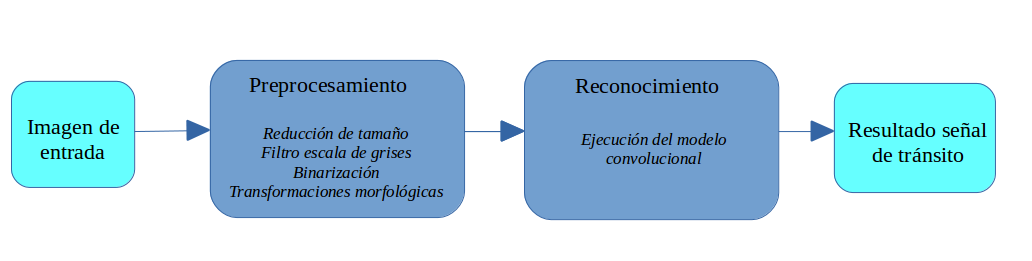
\includegraphics[width=0.8\textwidth]{images/intro/bloque}
		\end{center}
		\begin{center}
		\caption{\small{Diagrama de bloques para el reconocimiento}}
		{\small{Fuente: Elaboración propia}}
		\end{center}
		\vspace{-1.5em}
		\end{figure}

	\end{itemize}
	}
%-------------------------------------------------------------------------------------------------
%-------------------------------------------------------------------------------------------------



\section{Contribución de la investigación}
\frame{
\begin{block}
{\Large{Contribución de la investigación}}
\end{block}
\vskip 0.5cm
\begin{itemize}
\item<1->Todos los hechos descritos hacen que el reconocimiento de las señales de tránsito sea un reto desafiante y esencial en muchos aspectos, no solo para contribuir en los esfuerzos de la industria automotriz en el campo de la asistencia al conductor, sino también para organismos internacionales y gubernamentales  que buscan constantemente introducir nuevos mecanismos y tecnologías que faciliten y mejoren la conducción vehicular. Es por ello que esta investigación contribuye de la siguiente manera:
\end{itemize}
}




\frame{
\begin{block}
{\Large{Contribución de la investigación}}
\end{block}
\vskip 0.5cm
\begin{itemize}
\item<1-> Otorga un modelo computacional para el reconocimiento de 43 tipos de señales de Tránsito de Alemania, con una tasa de acierto del {\bf 98.62\%}, mucho mejor que el resultado obtenido por \citep{Ayuque2016} - 95.29\% y mucho más próximo al mejor resultado obtenido en las investigaciones hechas en base al dataset GTSRB (99.46\% - \citep{Ciresan}).
\vskip 0.5cm
\item<2-> Otorga un modelo computacional para el reconocimiento de 7 tipos señales de Tránsito del Perú, el cual posee un {\bf(99.83\%)} de acierto tras analizar una muestra de 4698 imágenes. 
\vskip 0.5cm
\item<3-> La investigación ofrece para futuras investigaciones, un dataset de señales de Tránsito del Perú compuesto por 31314 imágenes distribuidas en 7 categorías.
\end{itemize}
}

%-------------------------------------------------------------------------------------------------
%-------------------------------------------------------------------------------------------------

